% Compile with:  pdflatex docs/model2_explained.tex   (run twice for the TOC)
% Only standard packages -- no bibliography, no external images.
\documentclass[11pt,a4paper]{article}

\usepackage[margin=2.4cm]{geometry}
\usepackage{booktabs}
\usepackage{amsmath}
\usepackage{amssymb}
\usepackage{xcolor}
\usepackage{tikz}
\usetikzlibrary{positioning, arrows.meta, fit, backgrounds}
\usepackage[colorlinks=true, linkcolor=blue!50!black, urlcolor=blue!50!black]{hyperref}
\usepackage{titlesec}
\usepackage{enumitem}
\usepackage{fancyhdr}

\titleformat{\section}{\Large\bfseries\color{blue!35!black}}{\thesection}{0.6em}{}
\titleformat{\subsection}{\large\bfseries\color{blue!25!black}}{\thesubsection}{0.6em}{}
\setlist{itemsep=2pt, topsep=4pt}
\pagestyle{fancy}\fancyhf{}
\fancyhead[L]{\small MMF-Net --- what we built and why}
\fancyfoot[C]{\thepage}
\renewcommand{\headrulewidth}{0.4pt}

\newcommand{\good}[1]{\textcolor{green!45!black}{\textbf{#1}}}
\newcommand{\bad}[1]{\textcolor{red!65!black}{\textbf{#1}}}

\title{\vspace{-1.5cm}\textbf{MMF-Net: A Graph-Free Multimodal Transformer\\for Flood Early Warning in Sri Lanka}\\[0.3cm]
\large What we built, why each piece is there, and why it beats the graph model}
\author{Sri Lanka Flood Early-Warning Project --- Model 2}
\date{August 2026}

\begin{document}
\maketitle
\thispagestyle{fancy}

\begin{abstract}
\noindent
This document explains \textbf{Model 2 (MMF-Net)}, the second of two neural
architectures built for this project, and why it outperforms \textbf{Model 1
(TF-STGNN)}, the graph neural network we built first. MMF-Net reaches a test
PR-AUC of \good{0.8355} against Model 1's 0.7421 --- and it does so
\emph{without a graph}, with a comparable parameter count. The single largest
gain in the whole project came not from a new architecture but from changing
how each input number enters the network. The second largest came from
\emph{removing} a loss function that everyone recommends for imbalanced data.
Both are documented here with controlled, one-variable-at-a-time evidence.
\end{abstract}

\tableofcontents
\vspace{0.5cm}

% ============================================================================
\section{The problem, in one page}

\subsection{What we are predicting}

For each of \textbf{51 river monitoring points} across \textbf{16 basins} in Sri
Lanka, on each day, we predict:

\begin{center}
\emph{Will tomorrow's river discharge at this point exceed its
98\textsuperscript{th} percentile?}
\end{center}

That is the primary target, \texttt{target\_flood\_1d}. The network also
predicts five auxiliary targets at the same time (flooding in 2 and 3 days, the
\emph{onset} of a new flood tomorrow, and two continuous discharge quantities),
because forcing one representation to serve several related questions is a
cheap form of regularisation.

\subsection{Why this is hard}

\begin{table}[h]
\centering
\small
\begin{tabular}{@{}lp{10.5cm}@{}}
\toprule
\textbf{Difficulty} & \textbf{What it means in practice} \\
\midrule
Severe class imbalance & Only \textbf{2.0\%} of node-days are floods. A model
that always says ``no flood'' is 98\% accurate and completely useless. This is
why we never report accuracy. \\[3pt]
Few \emph{independent} examples & Those 2\% are not independent. They come from
\textbf{1,469 flood episodes} averaging 5.4 days each, and one storm floods many
nodes at once. The effective sample size is far smaller than the row count. \\[3pt]
Strong autocorrelation & If a river is flooding today, it is probably flooding
tomorrow. A naive evaluation rewards a model for noticing an ongoing flood
rather than for predicting a new one. \\[3pt]
A quiet validation period & Our validation years (2018--2020) had only 0.81\%
flood days versus 2.28\% in test. Validation scores therefore look much worse
than test scores and the two are not comparable. \\
\bottomrule
\end{tabular}
\end{table}

\subsection{The data}

A dense tensor of $8{,}036 \text{ days} \times 51 \text{ nodes} \times 33
\text{ features}$ (rainfall, soil moisture, temperature, discharge and their
lagged aggregates), plus 9 static terrain features per node.

\begin{table}[h]
\centering
\small
\begin{tabular}{@{}lllr@{}}
\toprule
\textbf{Split} & \textbf{Years} & \textbf{Valid node-days} & \textbf{Flood days} \\
\midrule
Train      & 2003--2017 & 277,899 & 2.028\% \\
Validation & 2018--2020 & 55,896  & 0.810\% \\
Test       & 2021--2024 & 74,463  & 2.276\% \\
\bottomrule
\end{tabular}
\end{table}

The split is \textbf{chronological}. Everything the model sees during training
happened before everything it is tested on --- which is the only honest setup
for a forecasting problem, and Section~\ref{sec:leakage} shows what happens when
you get this wrong.

% ============================================================================
\section{The two models at a glance}

\begin{table}[h]
\centering
\small
\begin{tabular}{@{}p{3.1cm}p{5.2cm}p{5.6cm}@{}}
\toprule
& \textbf{Model 1 --- TF-STGNN} & \textbf{Model 2 --- MMF-Net} \\
\midrule
Idea & Rivers form a network, so use a graph neural network to pass information
between connected nodes.
& Make the \emph{per-node} model as strong as possible, and see whether the
graph is still needed. \\[3pt]
Input layer & The 33 features enter as raw numbers into a linear layer.
& Each feature gets its \textbf{own learned embedding} (periodic + linear). \\[3pt]
Time encoder & 2-layer GRU with attention pooling.
& 3-layer Transformer over the 14-day window. \\[3pt]
Feature mixing & One linear layer.
& \textbf{Attention across the 33 channels}. \\[3pt]
Spatial structure & Relational GATv2 over 290 edges (35 directed flow, 204
spatial, 51 self-loops).
& \textbf{None, by design.} \\[3pt]
Terrain & FiLM conditioning. & FiLM conditioning (kept --- it worked). \\[3pt]
Satellite imagery & ResNet-18, embedding \emph{concatenated}.
& ResNet-18, embedding fused through a \textbf{learned gate}. \\[3pt]
Parameters & 581,319 & 710,870 \\[3pt]
\textbf{Test PR-AUC} & 0.7421 & \good{0.8355} \\
\bottomrule
\end{tabular}
\end{table}

\noindent
Both models read the same 33 channels, use the same train/val/test split, the
same loss code, the same metrics code and the same training loop (all in the
shared \texttt{floodlib} package). \textbf{Any difference between them is a
difference of architecture, never of evaluation.} That was a deliberate design
decision --- if each model owned a copy of the evaluation code, a comparison
between them would silently become a comparison of protocols.

% ============================================================================
\section{Model 2, stage by stage}

\begin{figure}[h]
\centering
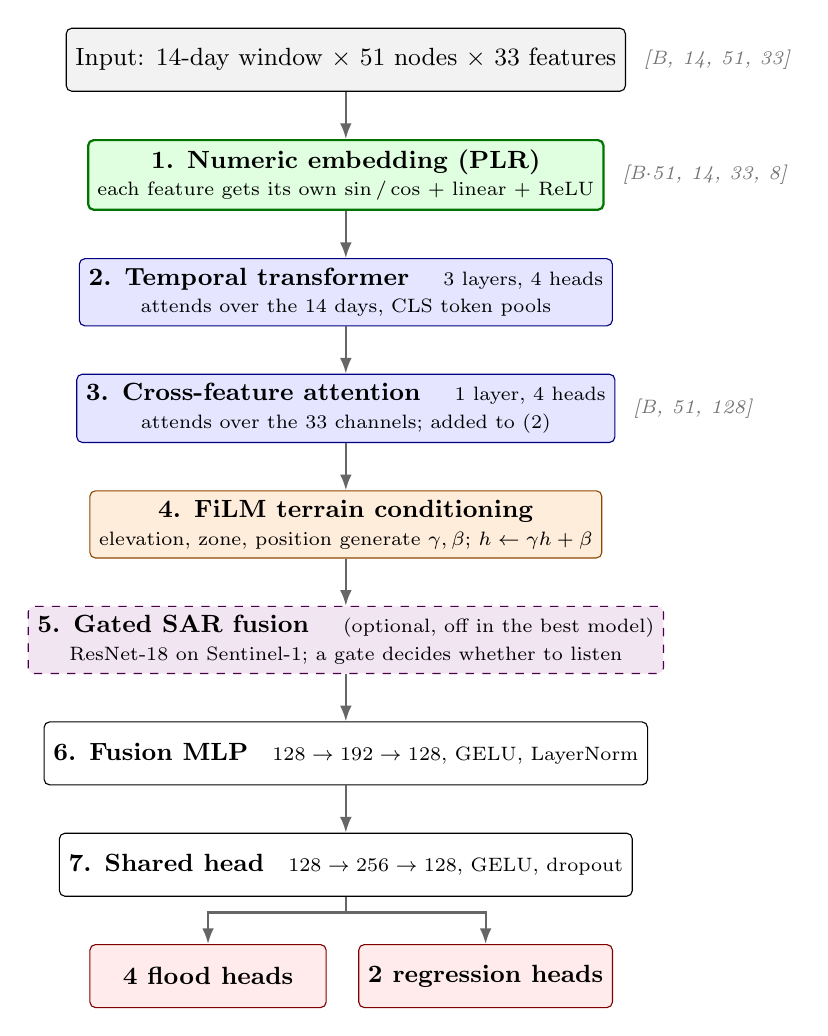
\begin{tikzpicture}[
  node distance=6mm,
  box/.style={draw, rounded corners=2pt, align=center, minimum width=6.4cm,
              minimum height=8mm, font=\small, fill=white},
  hl/.style={box, fill=green!12, draw=green!45!black, thick},
  dim/.style={font=\scriptsize\itshape, text=black!55},
  arr/.style={-{Latex[length=2mm]}, thick, black!60}
]
\node[box, fill=black!5] (in) {Input: 14-day window $\times$ 51 nodes $\times$ 33 features};
\node[dim, right=1mm of in] {[B, 14, 51, 33]};

\node[hl, below=of in] (emb) {\textbf{1. Numeric embedding (PLR)}\\[-1pt]
  {\scriptsize each feature gets its own $\sin/\cos$ + linear + ReLU}};
\node[dim, right=1mm of emb] {[B$\cdot$51, 14, 33, 8]};

\node[box, fill=blue!10, draw=blue!50!black, below=of emb] (tt)
  {\textbf{2. Temporal transformer} \quad {\scriptsize 3 layers, 4 heads}\\[-1pt]
  {\scriptsize attends over the 14 days, CLS token pools}};

\node[box, fill=blue!10, draw=blue!50!black, below=of tt] (fa)
  {\textbf{3. Cross-feature attention} \quad {\scriptsize 1 layer, 4 heads}\\[-1pt]
  {\scriptsize attends over the 33 channels; added to (2)}};
\node[dim, right=1mm of fa] {[B, 51, 128]};

\node[box, fill=orange!14, draw=orange!55!black, below=of fa] (film)
  {\textbf{4. FiLM terrain conditioning}\\[-1pt]
  {\scriptsize elevation, zone, position generate $\gamma,\beta$; $h \leftarrow \gamma h + \beta$}};

\node[box, fill=violet!10, draw=violet!60!black, dashed, below=of film] (sar)
  {\textbf{5. Gated SAR fusion} \quad {\scriptsize (optional, off in the best model)}\\[-1pt]
  {\scriptsize ResNet-18 on Sentinel-1; a gate decides whether to listen}};

\node[box, below=of sar] (fuse) {\textbf{6. Fusion MLP} \; {\scriptsize $128 \to 192 \to 128$, GELU, LayerNorm}};
\node[box, below=of fuse] (head) {\textbf{7. Shared head} \; {\scriptsize $128 \to 256 \to 128$, GELU, dropout}};

\node[box, fill=red!8, draw=red!50!black, below=of head, minimum width=3.0cm, xshift=-1.75cm] (cls)
  {\textbf{4 flood heads}};
\node[box, fill=red!8, draw=red!50!black, minimum width=3.0cm, right=4mm of cls] (reg)
  {\textbf{2 regression heads}};

\draw[arr] (in) -- (emb);
\draw[arr] (emb) -- (tt);
\draw[arr] (tt) -- (fa);
\draw[arr] (fa) -- (film);
\draw[arr] (film) -- (sar);
\draw[arr] (sar) -- (fuse);
\draw[arr] (fuse) -- (head);
\draw[arr] (head.south) -- ++(0,-2mm) -| (cls.north);
\draw[arr] (head.south) -- ++(0,-2mm) -| (reg.north);
\end{tikzpicture}
\caption{MMF-Net. Green is where the largest gain came from. The dashed block is
disabled in the best configuration.}
\end{figure}

\subsection{Stage 1 --- numeric embedding (the important one)}

\textbf{The problem it solves.} Neural networks are famously worse than
gradient-boosted decision trees on tabular data, and our Model 1 result showed
exactly that: 0.7421 against the tree baseline's 0.8496. The published
explanation is that the \emph{input layer}, not the depth of the network, is
what loses. A decision tree can split on ``rainfall $>$ 47\,mm'' for free; a
linear layer fed a raw number has to approximate that sharp boundary with a
smooth function, and it is bad at it.

\textbf{What we do instead.} Feature $j$ with value $x$ becomes
\[
  \mathbf{e}_j(x) \;=\; \mathrm{ReLU}\!\Big(
     W_j \big[\, \sin(2\pi c_j x),\; \cos(2\pi c_j x) \,\big] + b_j \Big)
     \;\in\; \mathbb{R}^{8},
\]
where $c_j \in \mathbb{R}^{8}$ are \emph{learned frequencies}, one set per
feature, and $W_j$ is a per-feature projection. The periodic expansion lets the
network represent a sharp threshold in a scalar --- the thing it could not do
before. Frequencies start small ($\sigma = 0.05$); large initial frequencies
alias the input and the model never recovers.

\textbf{What it bought.} Changing \emph{only} this, from a plain linear
embedding to the periodic one:

\begin{center}
\small
\begin{tabular}{@{}llll@{}}
\toprule
& \textbf{PR-AUC} & \textbf{Event detection} & \textbf{Everything else} \\
\midrule
N0 (linear embedding)  & 0.6083 & 0.290 & identical \\
N1 (periodic embedding) & \good{0.7605} & \good{0.420} & identical \\
\midrule
\textbf{Difference} & \textbf{+0.1522} & \textbf{+0.130} & --- \\
\bottomrule
\end{tabular}
\end{center}

\noindent
\textbf{This is the largest single change in the entire project}, larger than
FiLM ($+0.105$), larger than the ensemble, larger than anything in Model 1.

\subsection{Stage 2 --- temporal transformer}

Each day's 33 embedded features are flattened and projected to a single
128-dimensional token. A learned \texttt{CLS} token and learned positional
embeddings are prepended, and a 3-layer pre-LayerNorm Transformer (4 heads,
feed-forward width 256, GELU, dropout 0.2) attends over the resulting 15 tokens.
The \texttt{CLS} output is the node's summary.

\textbf{Why attention rather than the GRU.} A recurrent network has to carry the
memory of a rainfall event forward through 14 sequential steps. Attention can
look straight back at the day the rain fell. As a bonus, the \texttt{CLS}
token's attention row is directly readable as the rainfall-to-discharge lag.

\textbf{An honest caveat.} Comparing the two floors --- M0 (GRU, 0.5981) against
N0 (transformer, 0.6083) --- the transformer \emph{by itself} bought only
$+0.010$. \textbf{The win came from the input layer, not the sequence model.}
That is a more interesting finding than ``transformers are better'', and it is
what the tabular deep-learning literature predicts.

\subsection{Stage 3 --- cross-feature attention}

The temporal transformer mixes the 33 features through a single linear
projection, which cannot express \emph{``this much rain matters only when the
soil is already wet''}. So we take the per-feature embeddings, average them over
the 14 days, and run one more attention layer \emph{across the 33 channels}.

Averaging over time first is what makes this affordable: 33 tokens per node-day
instead of $33 \times 14$. Gain: $+0.0133$ (N1 $\to$ N2). Small --- see
Section~\ref{sec:caveats}.

\subsection{Stage 4 --- FiLM terrain conditioning}

The 9 static terrain features (elevation, log drainage area, climate zone
one-hot, upstream/downstream position one-hot) do not enter as 9 extra input
columns. Instead a small network turns them into a scale $\gamma$ and a shift
$\beta$, and the node's temporal state is modulated:
\[
h \leftarrow \mathrm{LayerNorm}\big(h \odot (1+\gamma) + \beta\big).
\]
\textbf{Why this rather than concatenation.} Terrain does not \emph{add}
evidence about flooding --- it changes \emph{how to read} the evidence. The same
50\,mm of rain means something different on a steep wet-zone headwater than on a
flat dry-zone outlet. Multiplication expresses that; concatenation does not. The
final layer is zero-initialised so $\gamma = \beta = 0$ at the start, which makes
the conditioned model a strict superset of the unconditioned one.

Gain: $+0.105$ in Model 1 (M0 $\to$ M1), $+0.053$ in Model 2 (N2 $\to$ N3).
Replicated in both families.

\subsection{Stage 5 --- gated SAR fusion (disabled in the best model)}

Sentinel-1 radar sees through cloud, which optical imagery cannot. But it
revisits only every $\sim$12 days, and our built dataset covers only \textbf{9 of
the 51 nodes}. So on the overwhelming majority of node-days there is no image.

Model 1 concatenated the image embedding into a fixed slot, which forces the
network to distinguish ``no water'' from ``no picture'' on every single sample.
Model 2 uses a gate instead:
\[
g = \sigma\big(\mathrm{MLP}[\,h;\, v;\, \text{present};\, \text{age}/30\,]\big),
\qquad
h \leftarrow \mathrm{LayerNorm}\big(h + g \odot W v \odot \text{present}\big).
\]
The gate is zero-initialised with a $-3$ bias so it starts shut, and the
\text{present} factor means an absent frame contributes exactly nothing.
See Section~\ref{sec:negative} for the outcome.

\subsection{Stages 6--7 --- fusion, head, and the six outputs}

A two-layer fusion MLP ($128 \to 192 \to 128$) and a shared head
($128 \to 256 \to 128$) feed two output layers: four flood-classification heads
and two regression heads. Predictions from \textbf{5 independently seeded models}
are averaged in probability space, and a single temperature parameter --- fitted
on validation only, then frozen --- calibrates them.

\textbf{Total: 710,870 parameters.}

% ============================================================================
\section{The experiments}

Every rung of the ladder changes \textbf{exactly one thing} from the rung above,
so any difference is attributable.

\begin{table}[h]
\centering
\small
\begin{tabular}{@{}llrrrrr@{}}
\toprule
\textbf{Run} & \textbf{Change from the row above} & \textbf{PR-AUC} & \textbf{ev.det} & \textbf{FAR} & \textbf{ECE} & \textbf{Params} \\
\midrule
N0 & floor: linear feature embeddings & 0.6083 & 0.290 & 0.412 & 0.0024 & 551k \\
N1 & \textbf{+ periodic (PLR) embeddings} & \good{0.7605} & 0.420 & 0.325 & 0.0053 & 555k \\
N2 & + cross-feature attention & 0.7738 & 0.423 & 0.313 & 0.0056 & 693k \\
N3 & + FiLM terrain & 0.8269 & 0.197 & 0.110 & 0.0032 & 711k \\
N4 & + focal $\times$ confidence loss & \bad{0.7592} & 0.220 & 0.138 & \bad{0.0525} & 711k \\
N5 & + 5-seed ensemble + temperature & 0.7846 & 0.208 & 0.145 & 0.0043 & 711k \\
\textbf{N5\_bce} & \textbf{the same, but on plain BCE} & \good{0.8355} & 0.220 & 0.120 & \good{0.0016} & 711k \\
N6\_scalars & + SAR summary statistics & 0.7284 & 0.397 & 0.344 & 0.0055 & 719k \\
N6\_gated & + gated SAR CNN & 0.8310 & 0.217 & 0.107 & 0.0066 & \bad{11,967k} \\
\bottomrule
\end{tabular}
\end{table}

\subsection{How to read the metrics}

\begin{table}[h]
\centering
\small
\begin{tabular}{@{}lp{11.2cm}@{}}
\toprule
\textbf{PR-AUC} & Precision--recall area under curve. \textbf{The headline
number.} At a 2\% positive rate, random guessing scores 0.02, so 0.8355 is a
$\sim$42$\times$ lift. Used instead of accuracy because ``never floods'' scores
98\%. \\[3pt]
\textbf{ev.det} & Event detection rate: the fraction of flood \emph{episodes}
where the model raised an alarm in the 7 days \emph{before} onset. An episode
detected once counts once --- this is what an operator actually experiences. \\[3pt]
\textbf{FAR} & False alarm ratio: of all the alarms raised, what fraction were
wrong. Lower is better. \\[3pt]
\textbf{ECE} & Expected calibration error: when the model says ``70\%'', does it
happen 70\% of the time? \textbf{Essential for a warning system} --- an
uncalibrated probability cannot support a decision threshold. \\[3pt]
\textbf{POD / CSI} & Probability of detection (recall) and critical success
index, the standard operational-meteorology scores. \\
\bottomrule
\end{tabular}
\end{table}

\noindent
\textbf{A warning about the ev.det column:} do not read it down the ladder. The
thresholds differ between rows (FAR ranges from 0.107 to 0.412), so it compares
\emph{operating points}, not models. N3 looks like a collapse against N2 only
because it is operating far more conservatively --- its threshold-free PR-AUC
went \emph{up}. Use \texttt{models/rethreshold.py} to force a common false-alarm
rate before comparing.

% ============================================================================
\section{Results: everything side by side}

\begin{table}[h]
\centering
\small
\begin{tabular}{@{}llrrr@{}}
\toprule
& \textbf{Model} & \textbf{PR-AUC} & \textbf{ev.det} & \textbf{Params} \\
\midrule
& \textit{Baselines} & & & \\
& gradient-boosted trees & 0.8496 & 0.161 & --- \\
& discharge percentile rule (operational bar) & 0.8164 & 0.223 & --- \\
& persistence & 0.5904 & 0.223 & --- \\
& climatology & 0.1083 & 0.515 & --- \\
\midrule
& \textit{Model 1 --- TF-STGNN} & & & \\
& M0 (GRU floor) & 0.5981 & 0.262 & 295k \\
& M3 (full graph, BCE) & 0.7039 & 0.380 & 581k \\
& M5 (best: ensemble + calibration) & 0.7421 & 0.344 & 581k \\
\midrule
& \textit{Model 2 --- MMF-Net} & & & \\
& N0 (transformer floor) & 0.6083 & 0.290 & 551k \\
& N3 (full, BCE, single seed) & 0.8269 & 0.197 & 711k \\
& \textbf{N5\_bce (best)} & \good{0.8355} & 0.220 & 711k \\
\bottomrule
\end{tabular}
\end{table}

\noindent
N5\_bce also holds the best Brier score (0.0080), ECE (0.0016), CSI (0.561) and
F1 (0.719) in the project, with a mean warning lead time of 5.45 days.

% ============================================================================
\section{Why Model 2 beats Model 1}

\subsection{Reason 1: a better input layer (the big one)}

Model 1 fed 33 raw numbers into a GRU. Model 2 gives each number its own learned
periodic embedding. \textbf{Isolated effect: $+0.152$ PR-AUC.} Everything else in
the comparison is secondary to this.

\subsection{Reason 2: the loss function was actively hurting}

Focal loss is the standard recommendation for class imbalance, and both ladders
adopted it by default. It was a mistake.

\begin{center}
\small
\begin{tabular}{@{}lrr@{}}
\toprule
& \textbf{PR-AUC} & \textbf{ECE} \\
\midrule
N3 --- plain BCE, single seed & 0.8269 & 0.0032 \\
N4 --- focal $\times$ confidence & \bad{0.7592} & \bad{0.0525} \\
N5 --- focal + ensemble + calibration & 0.7846 & 0.0043 \\
N5\_bce --- \textbf{BCE} + ensemble + calibration & \good{0.8355} & \good{0.0016} \\
\bottomrule
\end{tabular}
\end{center}

\noindent
N5 $\to$ N5\_bce changes \emph{only} the loss: $+0.0509$ PR-AUC, and calibration
error cut to a third.

\textbf{Why focal failed here.} Two mechanisms in the loss were fighting each
other. Focal loss says \emph{``concentrate the gradient on the examples you get
wrong''}. Our \texttt{label\_confidence} weighting says \emph{``the examples you
get wrong are the ones whose labels are unreliable''} --- it down-weights days
within $\pm 15\%$ of the flood threshold. Focal up-weights exactly what
confidence down-weights, and they cancel. On top of that, plain BCE is a
\emph{proper scoring rule} (its minimum is at the true probability) and focal is
not, so focal cannot be well calibrated by construction.

\textbf{This matters for Model 1 too:} M4, M5 and M6 all sit on the same rung, so
Model 1's published numbers are understated. An \texttt{M5\_bce} run would be a
fairer comparison.

\subsection{Reason 3: terrain conditioning, kept from Model 1}

FiLM was Model 1's single best idea and Model 2 kept it unchanged. It replicated:
$+0.105$ in Model 1, $+0.053$ in Model 2.

\subsection{Reason 4: the graph was not earning its place}

This is the finding Model 2 was built to test.

\begin{center}
\small
\begin{tabular}{@{}lrl@{}}
\toprule
& \textbf{PR-AUC} & \\
\midrule
M3 --- GRU \textbf{with} relational graph, BCE & 0.7039 & 581k params \\
N3 --- transformer, \textbf{no graph}, BCE & \good{0.8269} & 711k params \\
\bottomrule
\end{tabular}
\end{center}

\noindent
Within Model 1 the graph barely moved anything either: M1 (no graph) 0.7031
$\to$ M2 (spatial edges) 0.7148 $\to$ M3 (adding directed flow edges)
\emph{0.7039} --- adding the flow edges made it \emph{worse}.

\textbf{Why this is a legitimate finding and not a failure.} Model 1 could only
compare message passing against a \emph{weak} per-node floor (M0, a plain GRU).
Against a properly built per-node network, the graph adds nothing. There is
published support for this: river networks are tree-like, which causes
\emph{over-squashing} in GNNs --- information from many upstream nodes has to
squeeze through a single edge and is lost. A negative result on your own proposed
architecture, demonstrated against a strong alternative you also built, is worth
more than another incremental win.

% ============================================================================
\section{The negative results}
\label{sec:negative}

\begin{enumerate}[leftmargin=*]
\item \textbf{Message passing did not help.} Section 6.4.

\item \textbf{Focal loss hurt.} Section 6.2. Contrarian: this is the standard
recipe for imbalanced data.

\item \textbf{Satellite imagery added nothing.} N5\_bce, with \emph{no} imagery
and 711k parameters, beats N6\_gated, \emph{with} imagery and 11,967k
parameters (0.8355 vs 0.8310). What looked like a gain from vision was really
the BCE loss recovering what focal had destroyed. Diagnosis: a randomly
initialised ResNet-18 cannot learn what water looks like from a target with a
2\% positive rate, and the imagery reaches only 9 of the 51 nodes at a 12-day
revisit.
\end{enumerate}

% ============================================================================
\section{Leakage: the strongest methodological finding}
\label{sec:leakage}

We ran the identical model under a \emph{random} train/test split instead of a
chronological one:

\begin{center}
\small
\begin{tabular}{@{}lrr@{}}
\toprule
M3 under & \textbf{PR-AUC} & \textbf{Event detection} \\
\midrule
temporal split (honest) & 0.7039 & \good{0.380} \\
random split (leaky) & \bad{0.9050} & \bad{0.089} \\
\bottomrule
\end{tabular}
\end{center}

\noindent
A random split makes the model look \textbf{29\% better} while making it
\textbf{four times worse} at the job it exists to do. Day 3 of a flood ends up in
training and day 4 in test, so the model memorises rather than forecasts.

\textbf{Leakage does not merely inflate scores --- it inverts model selection.}
Anyone tuning on the random split would choose the wrong model.

% ============================================================================
\section{What is not yet established}
\label{sec:caveats}

Stated plainly, because a result you cannot defend is worse than no result.

\begin{enumerate}[leftmargin=*]
\item \textbf{Rungs N0--N4 are single-seed.} Across N5\_bce's five seeds, the
best validation episode PR-AUC ranged 0.3375--0.3856 --- a spread of 0.048. So
the $+0.152$ from periodic embeddings is safe (an order of magnitude larger), and
the $+0.051$ from the loss is safe (both sides are 5-seed), but the $+0.013$ from
cross-feature attention and the $+0.009$ from the ensemble \textbf{should not be
claimed} without per-seed error bars.

\item \textbf{The ev.det column is not comparable across rows} at differing false
alarm rates. It needs re-thresholding to a common FAR.

\item \textbf{The SAR encoder pretraining has never completed.} Three separate
bugs, all now fixed but not yet re-run, so ``can a CNN see flooding in Sentinel-1
at all?'' is formally untested. Our null result is about \emph{fusion}, not about
vision in principle.

\item \textbf{No embargo at the split boundary.} Targets look up to 3 days
forward, so a training day at the end of 2017 carries a label determined by
discharge in early 2018. A handful of rows, but worth checking in a project whose
headline finding is about leakage.

\item \textbf{Only one protocol for Model 2.} Model 1 was run under temporal,
basin-holdout and random splits; Model 2 only under temporal.
\end{enumerate}

% ============================================================================
\section{Summary}

\begin{enumerate}[leftmargin=*]
\item We built a graph neural network (Model 1), found it lost to a
gradient-boosted-tree baseline by 0.108 PR-AUC, and diagnosed this as the known
failure of neural networks on tabular data.

\item We built a \emph{graph-free} transformer (Model 2) whose defining feature
is that each input number gets its own learned periodic embedding. That single
change gained \textbf{+0.152 PR-AUC} --- the largest effect in the project.

\item We found the focal loss, adopted by default in both ladders as the standard
fix for class imbalance, was \textbf{actively harmful}: swapping it for plain BCE
gained another \textbf{+0.051} and cut calibration error to a third.

\item The final model, \textbf{N5\_bce}, reaches \textbf{PR-AUC 0.8355} at 711k
parameters --- beating Model 1 by 0.093, clearing the operational
discharge-percentile rule (0.8164), and closing \textbf{87\%} of the gap to the
tree baseline.

\item Along the way we produced three defensible negative results (message
passing, focal loss, satellite imagery) and one methodological finding (leakage
inverts model selection) that we consider the most valuable output of the
project.
\end{enumerate}

\end{document}
